%<dscrpt>Applications de la réécriture de listes.</dscrpt>
% <rel_id_type_rel>14</rel_id_type_rel> id de ``contient sans ordre l'élément''
% <rel_id_elt_parent>6469</rel_id_elt_parent> id de ``Algorithmique''

\begin{figure}
 \centering
 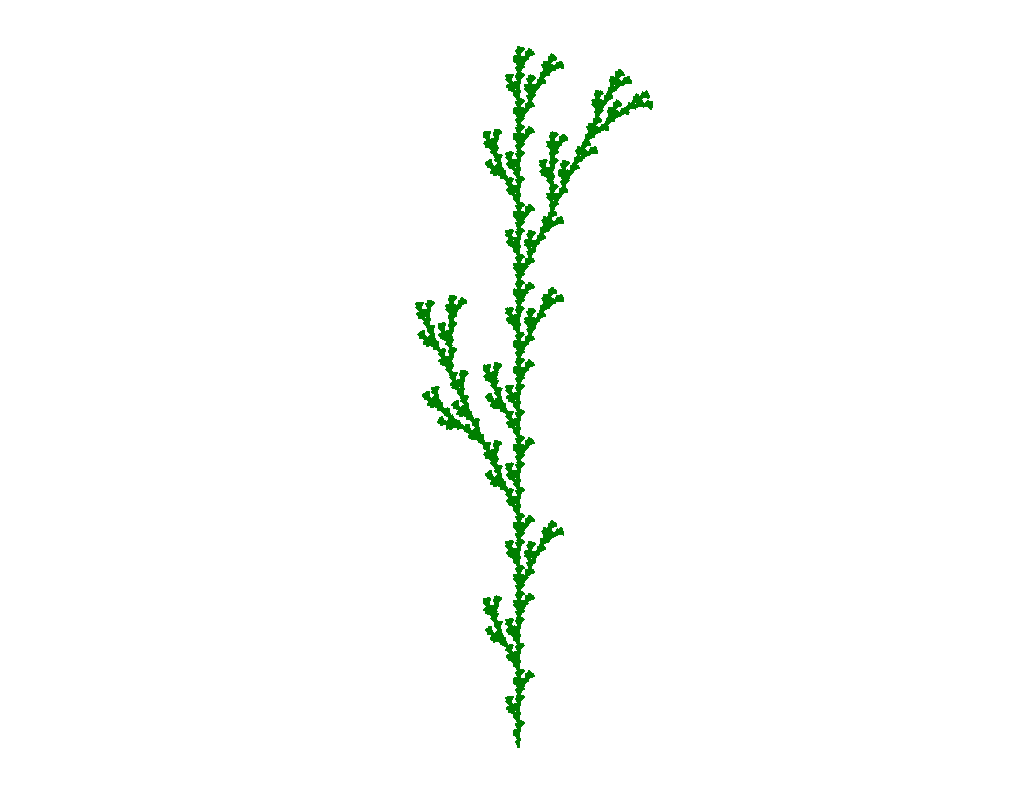
\includegraphics[width=8cm]{Ereecriture_1_fig.pdf}
 \caption{Une plante obtenue par réécriture de motifs}
 \label{fig:Ereecriture_1}
\end{figure}

L'objet de ce TP \footnote{d'après The Algorithmic Beauty of Plants (coll The Virtual Laboratory) Springer} est d'implémenter quelques applications de la réécriture non conditionnelle de listes\footnote{L-system}: d'abord au flocon de neige de Von Koch puis à la modélisation de plantes.\newline
On utilisera librement des modules Python sans se limiter au strict programme d'algorithmique. \newline
Le principe est de former une chaîne de caractères (d'abord avec les seuls caractères \verb|a|, \verb|l|, \verb|r| puis avec d'autres lettres encore) en partant d'une chaîne simple (\emph{initiateur}) et en substituant un \emph{motif} fixé à chaque occurence de \verb|a|. Cette substitution sera effectuée un certain nombre de fois suivant les capacités de la machine utilisée.\newline
Une chaîne de caractères permet de former un dessin lorsqu'elle est interprétée par une \emph{tortue traçante} qui se déplace dans le plan. Un \emph{état} de la tortue est un couple (direction, point).\newline
Chaque lettre est un ordre donné à la tortue. Les ordres sont interprétés de gauche à droite. Par exemple \verb|alaa| fait avancer puis tourner à gauche puis avancer deux fois. L'angle noté $\alpha$ est fixé.
\begin{itemize}
 \item la lettre \verb|l|  fait tourner sur place la tortue d'un angle $\alpha$ vers la gauche (dans le sens trigonométrique).
\item la lettre \verb|r|  fait tourner sur place la tortue d'un angle $\alpha$ vers la droite.
\item la lettre \verb|a|  fait avancer  la tortue de une fois son vecteur de direction et tracer le segment correspondant.
\end{itemize}
La structure de données utilisée pour représenter un état de la tortue est une liste de quatre nombres : les deux premiers sont les coordonnées de la direction, les deux derniers sont les coordonnées de la position.
\subsection*{Partie I. Flocons de Von Koch}
Dans cette partie, initialement la tortue est à l'origine du repère et dirigée suivant le premier vecteur de base. L'état initial est donc $[1,0,0,0]$. L'angle $\alpha$ est fixé à $\frac{\pi}{3}$. 
\begin{enumerate}
\item
\'Ecrire des fonctions désignées par \verb|a| , \verb|l| , \verb|r| dont l'argument \verb|E| désigne une liste de 4 nombres représentant l'état de la tortue.\newline
Les appels des fonctions \verb|l(E)|, \verb|r(E)| et \verb|a(E)| renvoient le nouvel état de la tortue après exécution de l'ordre correspondant. Placer ces fonctions dans un dictionnaire désigné par \verb|func_dic|; les clés sont les caractères \verb|a| , \verb|l| , \verb|r| et les valeurs sont les \emph{fonctions} de nom correspondant. 

 \item \begin{enumerate}
\item Former une \emph{chaîne de caractère} désignée par \verb|init| correspondant à la figure \ref{fig:Ereecriture_2} (triangle équilatéral). La position initiale est le sommet en bas à gauche et le premier segment est horizontal.

\begin{figure}[ht]
 \centering
 \begin{subfigure}[b]{4cm}
   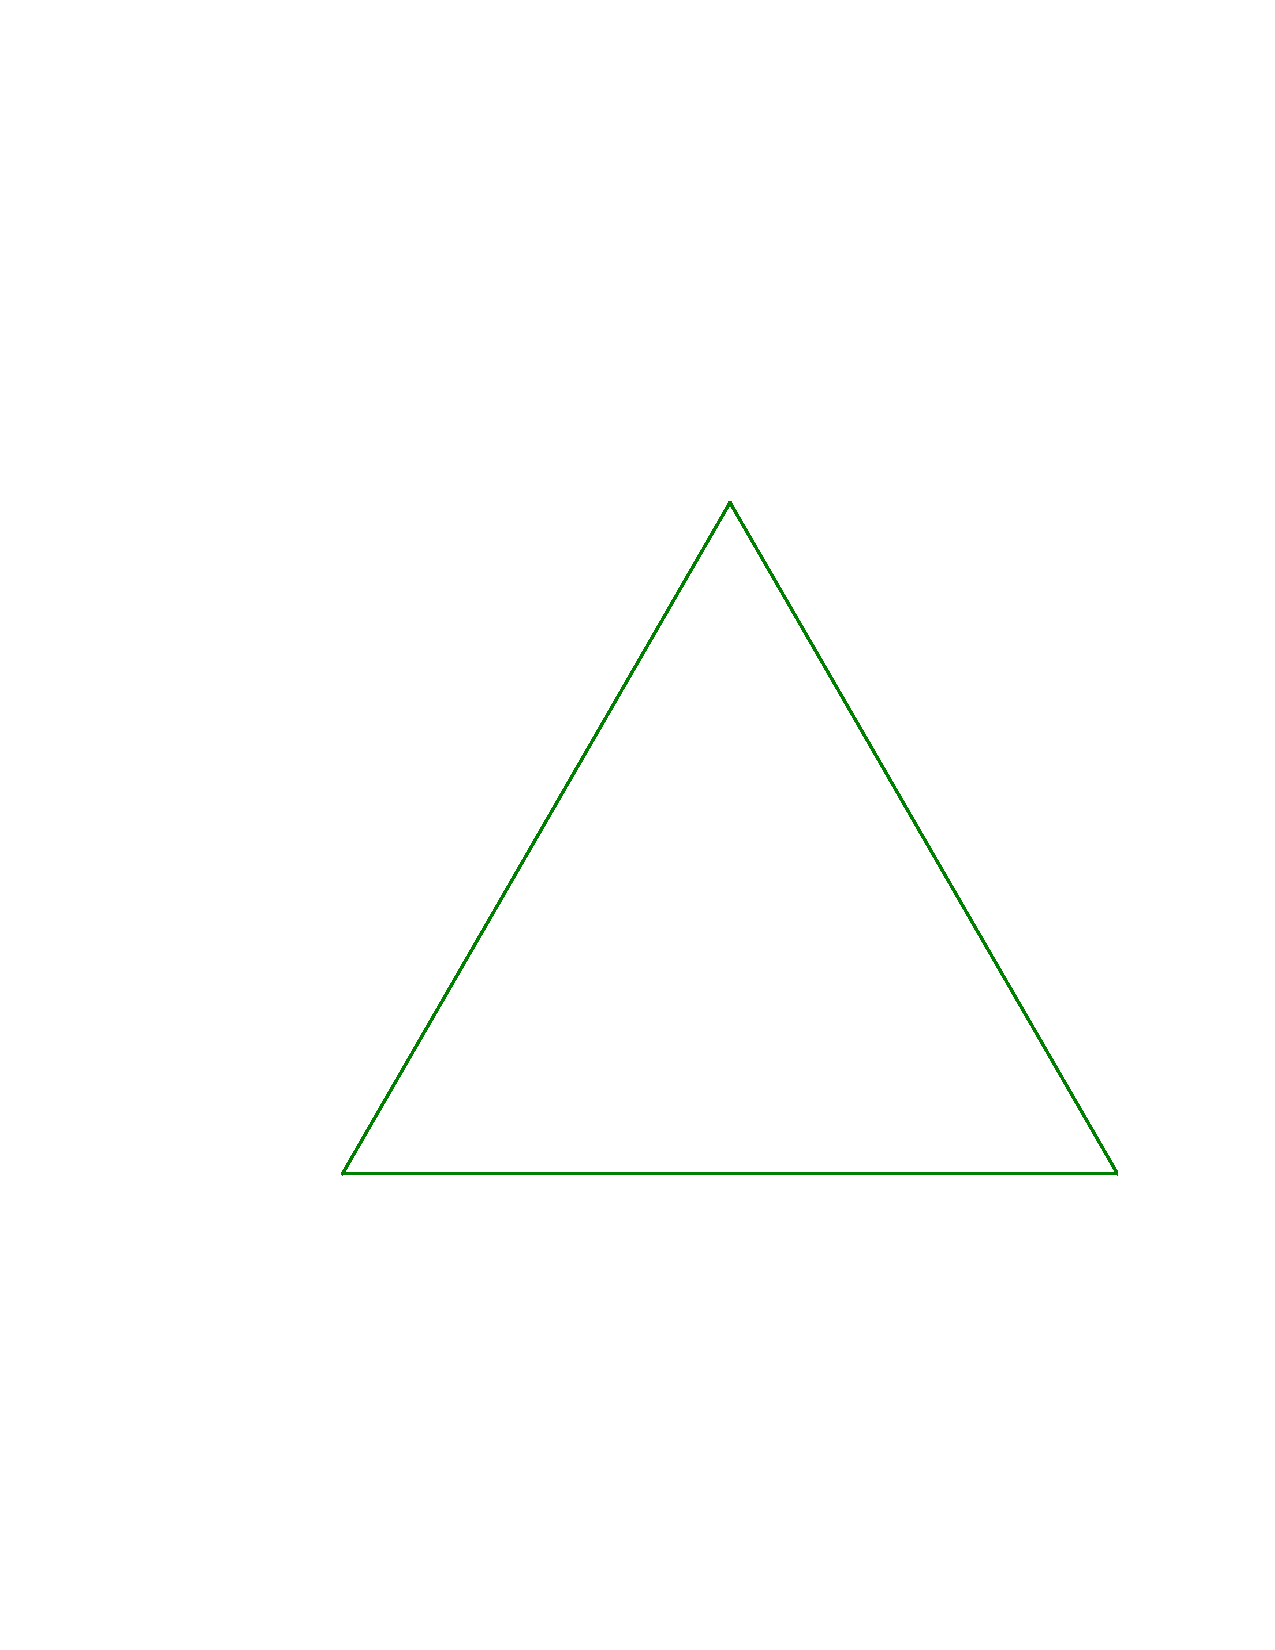
\includegraphics[width=3.5cm]{Ereecriture_2_fig.pdf}
   \caption{initiateur}  
 \end{subfigure} ~
 \begin{subfigure}[b]{4cm}
   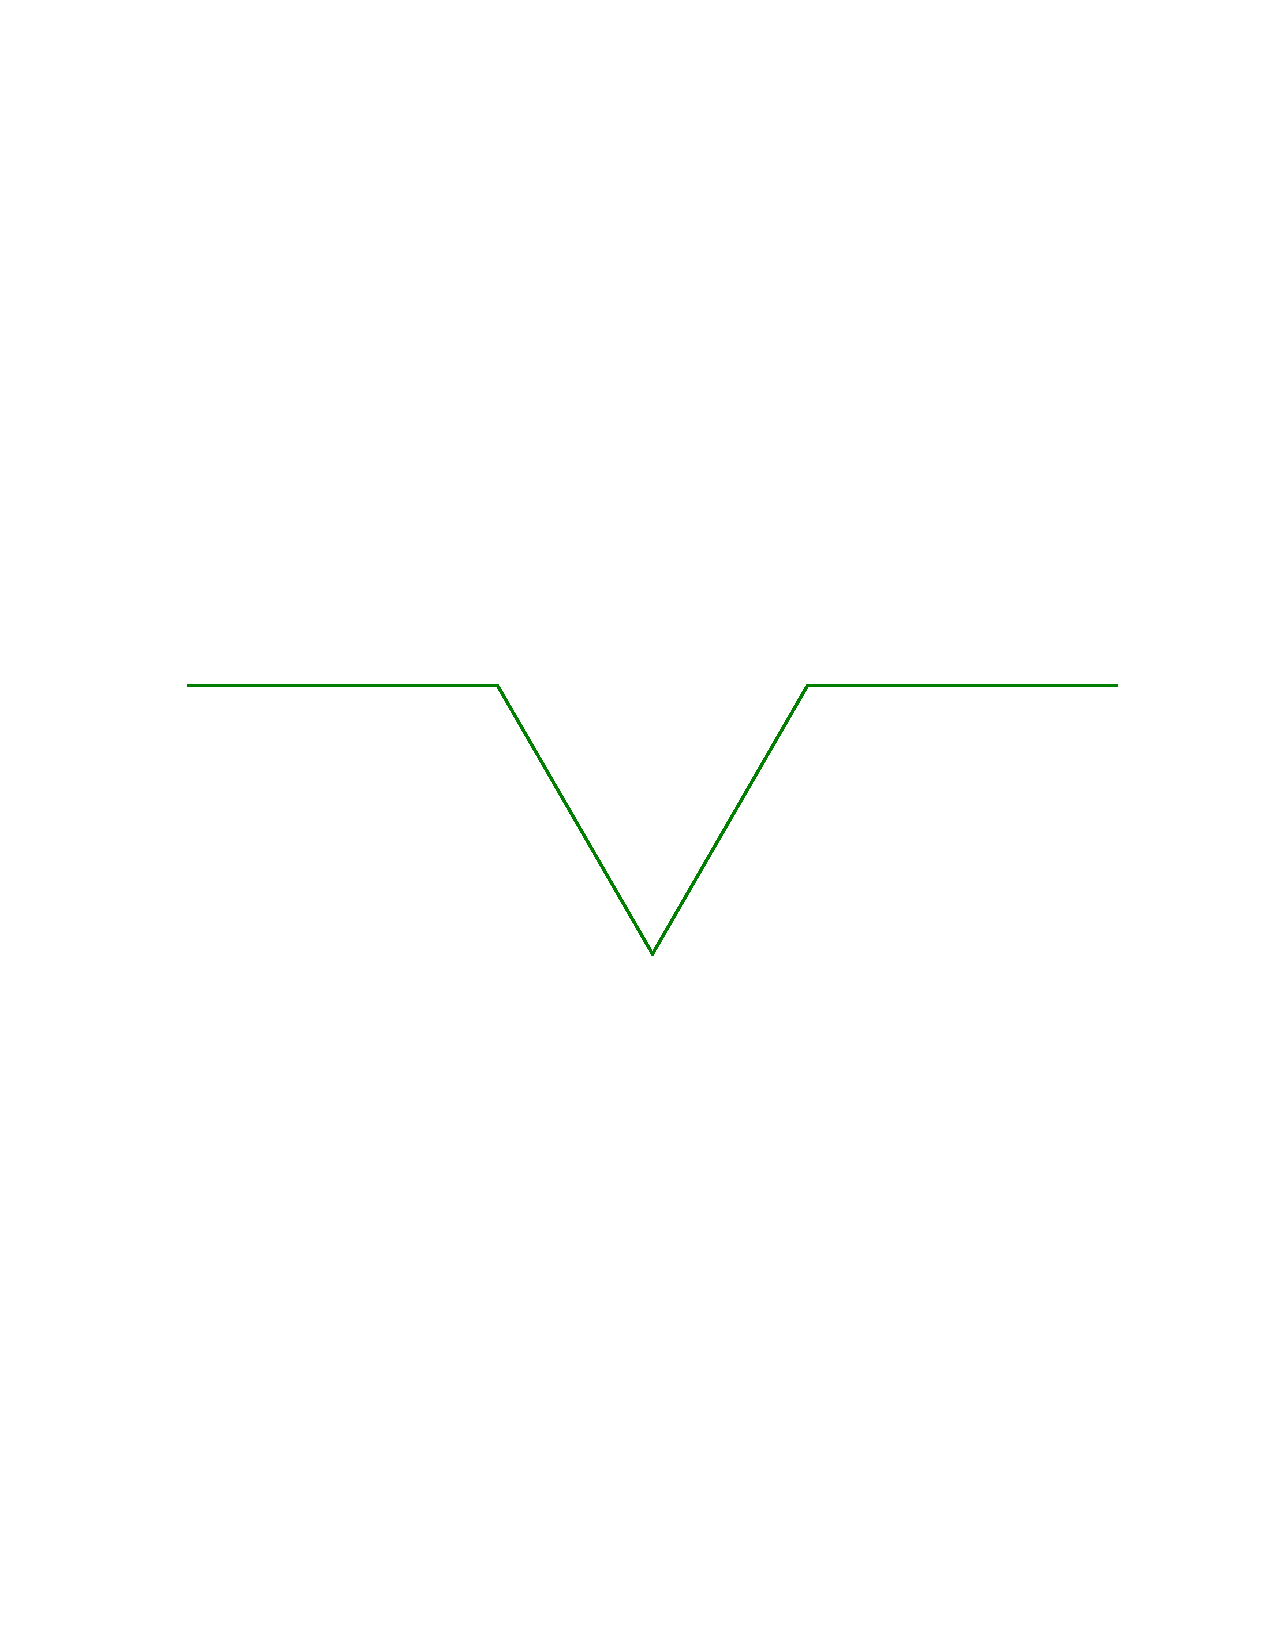
\includegraphics[width=3.5cm]{Ereecriture_3_fig.pdf}
   \caption{motif}\label{fig:Ereecriture_3} 
  \end{subfigure}
  \caption{Chaînes pour le flocon de Von Koch} \label{fig:Ereecriture_2}
\end{figure}

\item Former une chaîne de caractères désignée par \verb|motif| correspondant au dessin de la figure \ref{fig:Ereecriture_3}. La position initiale de la tortue étant tout à gauche.
\end{enumerate}

\item \'Ecrire une procedure \verb|affiche(L)| dont le paramètre \verb|L| désigne une chaîne de caractères et qui affiche le dessin correspondant. En reprenant \verb|L| et \verb|motif| trouvés en  2., vérifier que \verb|affiche(init)| et \verb|affiche(motif)| forment bien les dessins voulus. Il est utile de remarquer que tout caractère \verb|lettre| de \verb|L| est aussi le nom d'une fonction. On peut appeler cette fonction en utilisant le dictionnaire.

\item En reprenant \verb|init| et \verb|motif| trouvés en  2., assigner à \verb|L| le résultat de la substitution dans \verb|init| de \verb|a| par \verb|motif|. On pourra utiliser la méthode \verb|replace| des chaines de caractères. Recommencer quelques fois cette opération et former le dessin correspondant.
\end{enumerate}

\subsection*{Partie II. Dessins de plantes}
Pour former des dessins comme celui de la figure \ref{fig:Ereecriture_1}, il est nécessaire que la tortue puisse retourner (sans tracer de segment) à un de ses états précédents.\newline
Pour cela, on va introduire deux nouveaux caractères : \verb|(| et \verb|)| attachés à des fonctions \verb|e| (enregistre) et \verb|m| (se souvient).\newline
On va aussi changer de structure de données. Au lieu d'un état de la tortue, on va maintenant considérer une \emph{pile} d'états implémenter par une \emph{liste}. Le dernier état de cette liste est l'état \og actuel\fg, les autres sont des états plus anciens. Les ordres \verb|a|, \verb|l|, \verb|r| agissent exactement comme dans la partie I mais seulement sur l'état actuel de la tortue (le dernier), les autres état de la liste étant inchangés.\newline
Le nouvel ordre \verb|e| agit sur la liste en insérant l'état actuel à la fin de la liste. L'état actuel se retrouve alors deux fois en fin de liste ce qui revient à l'enregistrer.\newline
La fonction \verb|m| supprime le dernier état de la liste. L'état actuel devient alors celui qui était l'avant dernier.\newline
Les opérations \verb|e| et \verb|m| traduisent la propriété \og dernier entré premier sorti\fg\footnote{LIFO: Last In First Out} caractéristique d'une pile.\newline
Par exemple : effet de \verb|e|
\begin{displaymath}
 [E_1,E_2,E_3,E_4] \rightarrow [E_1,E_2,E_3,E_4,E_4]
\end{displaymath}
Effet de \verb|m|, la tortue à la faculté de se replacer dans état mémorisé le plus récent
\begin{displaymath}
 [E_1,E_2,E_3,E_4] \rightarrow [E_1,E_2,E_3]
\end{displaymath}

\begin{enumerate}
 \item Réécrire les procédures \verb|a(lE)|, \verb|l(lE)|, \verb|r(lE)| l'argument est maintenant une \emph{liste d'états} (nommée \verb|lE|) de la tortue mais elles ont les mêmes fonctions que dans la première partie.
\item \'Ecrire les procédures \verb|e(lE)| et \verb|m(lE)|.
\item Réécrire la procedure \verb|affiche(L)| pour l'adapter au nouveau contexte.\\Vérifier avec le flocon de Von Koch.
\item Initialiser maintenant verticalement la direction de la tortue. Reproduire les modèles de développement de plantes issus de l'ouvrage cité en note (les angles sont en degré):
\begin{displaymath}
% use packages: array
\renewcommand{\arraystretch}{1.2}
\begin{array}{l|l|l}
\text{initiateur} & \text{motif} & \text{angle} \\ \hline
a & a(la)a(ra)a & 25.7 \\ 
a & a(la)a(ra)(a) & 20 \\ 
a & aar(ralala)l(larara) & 22.5
\end{array}
\end{displaymath}
\item On obtient des modèles plus réalistes en introduisant encore une nouvelle lettre \verb|x| représentant un \emph{apex}. Un apex est un point de la plante où se forment les modifications : par exemple une nouvelle ramification. La substitution porte alors sur deux lettres simultanément. La lettre \verb|a| est remplacée par \verb|aa| (la tige grandit) et la lettre \verb|x| est remplacée par un mot \verb|motifx| qui peut être compliqué. Le mot initial est seulement le caractère \verb|x|. \newline
Que doit-on faire pour implémenter cette nouvelle structure ?\newline
Reproduire les modèles suivants :
\begin{displaymath}
% use packages: array
\renewcommand{\arraystretch}{1.2}
\begin{array}{l|l|l}
\text{initiateur} & \text{motifx} & \text{angle} \\ \hline
x & a(lx)a(rx)lx & 20 \\ 
x & a(lx)(rx)ax & 25.7 \\ 
x & ar((x)lx)la(lax)rx & 22.5
\end{array}
\end{displaymath}


\end{enumerate}
